\section{The quasimap mirror formula} \label{Section quasimap mirror theorem}

We are going to reproduce Gathmann's proof of the mirror formula with relative stable maps \cite{Ga-MF} in the context of quasimaps, thanks to the extension of his formula to this setting that we have proved in the previous sections. We have chosen to work with unparametrised quasimaps, hence the minimum number of markings is two; this minimal choice turns out to be extremely convenient because it determines the shape of the source curve to a high degree, so to grant a great level of control on degenerate contributions appearing in Gathmann's algorithm. The absence of rational tails in the quasimap moduli space makes the recursion much simpler, even in the CY case.

We would like to think of this as a Lefschetz-type theorem, in that it expresses certain (restricted) quasimap invariants of a hypersurface $Y$ in terms of those of the ambient space $X$. As it turns out, we have also retrieved a formula of Ciocan-Fontanine and Kim \cite[Corollary 5.5.1]{CF-K-wallcrossing} (but with more restrictive assumptions on the target); under this new light, the formula can be simply interpreted as a relation between some residues for the $\Gm$-action on the space of 0-pointed and 1-pointed \emph{parametrised} quasimap invariants of the hypersurface $Y$. It is remarkable how, knowing only about a small sector (i.e. invariants with few insertions), it is possible to formally reconstruct the full quasimap potential; a point which was greatly clarified to us by the discussion in \cite[Section 5.5]{CF-K-wallcrossing}.

We are going to be interested in the following \textbf{setup}: $X$ is a smooth projective toric variety and $Y$ is a smooth \emph{very ample} hypersurface in it, satisfying the following \emph{semi-positivity assumption}, that $-K_Y$ is nef. Notice that, by adjunction, it follows from our hypotheses that $-K_X$ is positive (at least) on every effective curve class \emph{coming from $Y$}. Let us denote by $r$ the dimension of $X$ and assume it is \emph{at least 3}. Then, in fact, every curve class on $X$ comes from $Y$ (by Lefschetz's hyperplane theorem) and $X$ \emph{is Fano}.

Denote dual bases for $H^*(X;\mathbb Q)$ by $\eta^i$ and $\eta_i$ ($i=0,\ldots,k$), with $\eta^0=\mathbbm 1_X$ and $\eta^1=Y$, which induce bases $\rho_i=i^*\eta_i$ for $i^*H^*(X)$ (extend it to a basis of $H^*(Y)$ by adding $\rho_{k+1}\ldots,\rho_{k'}$) and dually $\rho^i, i=1,\ldots,k'$; notice that the class of a point on $Y$ is given by restricting the dual of $\eta^1$, i.e. it is $\rho_1$, while the class of a point on $X$ is annihilated when restricted to $Y$, i.e. $\rho_0=0$. Furthermore, remark that, everytime we look at a relative space $\Q{0}{(m,0)}{X|Y}{\beta}$ with $m>0$, the evaluation map $\ev_1\colon \Q{0}{(m,0)}{X|Y}{\beta}\to X$ factors through $Y$ (so all the insertions can be first pulled back to $Y$).


\begin{dfn}
 Let $X$ be a smooth projective toric variety (or a complete intersection in a toric variety, or more generally any GIT quotient for which the quasimap spaces are defined), and consider 
 \[
  S_0^X(z,\beta)=(\ev_1)_*\left(\frac{1}{z-\psi_1}[\Q{0}{2}{X}{\beta}]^\text{vir}\right)
 \]
 %where $\ev_1$ is always thought of as landing in $\PP^r$.
 for every effective curve class $\beta\in H_2^+(X,\mathbb Z)$. Set $S_0^X(z,0)= \mathbbm 1_X$ and
 \[
  S_0^X(z,q)=\sum_{\beta\geq 0}S_0^X(z,\beta) q^\beta.
 \]
\end{dfn}

\begin{thm}
Let $X$ be a toric Fano variety of dimension at least 3, and $i\colon Y\subseteq X$ a very ample hypersurface such that $-K_Y$ is nef. Then
\begin{equation}\label{eqn:mirror}
   \frac{\sum_{\beta\geq 0} q^\beta\prod_{j=0}^{Y\cdot\beta}(Y+jz)S_0^X(z,\beta)}{P_0(q)}= i_*S_0^Y(z,q)
\end{equation}
where
\begin{align*}
 P_0(q)= & 1+\sum_{\substack{\beta>0\colon \\ K_Y\cdot\beta=0}} (Y\cdot\beta)q^\beta\langle [pt_Y],\mathbbm 1_{X}\rangle_{\Q{0}{(Y \cdot \beta,0)}{X|Y}{\beta}} \\
 = & 1+\sum_{\substack{\beta>0\colon \\ K_Y\cdot\beta=0}} q^\beta(Y\cdot\beta)!\langle\psi_1^{Y\cdot\beta-1}[pt_X],\mathbbm 1_{X}\rangle_{\Q{0}{2}{X}{\beta}}.
\end{align*}
\end{thm}

\begin{proof}

Define
 \[
  S_{0,(m)}^{X|Y}(z,\beta)=(\ev_1)_*\left(\frac{1}{z-\psi_1}[\Q{0}{(m,0)}{X|Y}{\beta}]^\text{vir}\right),
 \]
which coincides with the absolute $S_0$-function defined above for $m=0$, and
\[
 T_{(m)}^{X|Y}(z,\beta)=(\ev_1)_*\left(m[\Q{0}{(m,0)}{X|Y}{\beta}]^\text{vir}+\frac{1}{z-\psi_1}[D_m^{\mathcal Q}(X|Y,\beta)]^\text{vir}\right).
\]
Then, by Gathmann's formula, we can prove that
\begin{equation}\label{eqn:G}
 (Y+mz) S_{0,(m)}^{X|Y}(z,\beta) = S_{0,(m+1)}^{X|Y}(z,\beta)+ T_{(m)}^{X|Y}(z,\beta),
\end{equation}
from which it follows that
\[
 \prod_{j=0}^{Y\cdot\beta}(Y+jz) S_0^X(z,\beta) = \sum_{m=0}^{Y\cdot\beta}\prod_{j=m+1}^{Y\cdot\beta}(Y+jz)T_{(m)}^{X|Y}(z,\beta).
\]
It is now a matter of evaluating the RHS. Notice that $T_{(m)}^{X|Y}(z,\beta)$ is made of two parts:
\begin{itemize}[leftmargin=*]
 \item the \emph{boundary terms}: since there are only two markings and the first one is required to lie in $Y$, the strong stability condition for quasimaps forces the shape of the source curve to be that of a snake which the hypersurface cuts into two pieces, the internal one of degree $\beta^{(0)}$, and the external one of degree $\beta^{(1)}$ and multiplicity $m^{(1)}$ of contact with $Y$, with the first marked point belonging to the internal component and the second to the external one.

\begin{center}
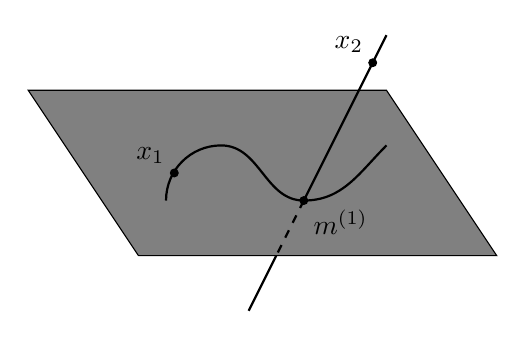
\begin{tikzpicture}[scale=0.7]
  \draw [fill=gray] (-.5,-1) -- (6,-1) -- (4,2) -- (-2.5,2) -- (-.5,-1);
  \draw [thick] (0,0) to [out=90,in=180] (1,1) to [out=0,in=180] (2.5,0) to [out=0,in=-135] (4,1);
  \draw [thick] (2.5,0) to (4,3);
  \draw [thick,dashed] (2.5,0) to (2,-1);
  \draw [thick] (2,-1) -- (1.5,-2);
  \draw [fill] (3.75,2.5) circle [radius=2pt] node[above left]{$x_2$};
  \draw [fill] (.15,.5) circle [radius=2pt] node[above left]{$x_1$};
  \draw [fill] (2.5,0.0) circle [radius=2pt] node[below right]{$m^{(1)}$};
 \end{tikzpicture}
\end{center}
 
 The invariants which we need to consider will hence be of the form
 \[
  \langle i^*\eta_i\psi_1^j,\rho^h\rangle_{\Q{0}{2}{Y}{\beta^{(0)}}}\langle \rho_h,\mathbbm 1_{X}\rangle_{\Q{0}{(m^{(1)},0)}{X|Y}{\beta^{(1)}}}, \quad h\in\{1,\ldots,k'\}
 \]
 
 Consider the following dimensional computation:
\begin{align*}
 0\leq \codim \rho^h &= \dim Y-\codim \rho_h \\
 &= \dim Y-\vdim \Q{0}{(m^{(1)},0)}{X|Y}{\beta^{(1)}} \\
 &= \dim Y-(\dim X-3-K_{X}\cdot \beta^{(1)}+2-m^{(1)})\\
 &= K_Y \cdot \beta^{(1)}-Y \cdot \beta^{(1)}+m^{(1)}\leq 0
\end{align*}
 where the last equality follows from adjunction, and the inequality follows from $K_Y\leq 0$ and $m^{(1)}\leq Y \cdot \beta^{(1)}$.
This shows that the only non-trivial contributions are due to the classes $\beta^{(1)}$ such that $K_Y \cdot \beta^{(1)}=0$, and the order of tangency is forced to be maximal, i.e. $m^{(1)}=Y \cdot \beta^{(1)}$. Furthermore, the only relevant insertions are $\rho^1=\mathbbm 1_Y$ and $\rho_1=[pt_Y]$. Finally, $m^{(1)}=Y \cdot \beta^{(1)}$ implies that
\[
 m=\alpha_1=Y \cdot \beta^{(0)}+m^{(1)}=Y \cdot \beta,
\]
hence the boundary contributions do not show up until the very end of the process of ``increasing the multiplicity''.

\item The remaining term in $T_{(m)}^{X|Y}(z,\beta)$ is $m(\ev_1)_*[\Q{0}{(m,0)}{X|Y}{\beta}]^\text{vir}$; notice that it only gets insertions from the cohomology of $X$ (restricted to $Y$). On the other hand
\[
 \vdim \Q{0}{(m,0)}{X|Y}{\beta}=\dim X-3 -K_X \cdot \beta +2-m \geq r-1
\]
because $m\leq Y\cdot\beta$ and $-(K_X+Y).\beta\geq 0$, by adjunction, projection formula, and for every effective curve class $\beta$ (coming from $Y$, but saying this is superfluous by Lefschetz's hyperplane theorem as we have already remarked); since the restriction of the class $[pt_X]$ to $Y$ vanishes, the only insertion that contributes is $\eta_1$ (by definition of a dual basis, all other dimension 1 classes vanish when restricted to $Y$), forcing the equality $m=Y\cdot\beta$, so that again this correction term is non-trivial only in the last step of the algorithm.
\end{itemize}
So, in the end, we see that equation \ref{eqn:G} reduces to
\begin{align*}
 &\prod_{j=0}^{Y\cdot\beta}(Y+jz) S_0^X(z,\beta) = T_{(Y\cdot\beta)}^{X|Y}(z,\beta) \\
 &= \sum_{i=1,\ldots,k;j\geq 0}z^{j+1}\eta^i\langle \rho_i\psi_1^j,\mathbbm 1_{Y}\rangle_{\Q{0}{2}{Y}{\beta}} \\
 &+\sum_{\substack{0<\beta^{(0)}<\beta \\ \beta^{(0)}+\beta^{(1)}=\beta}}z^{j+1}\eta^i\langle \rho_i\psi_1^j,\mathbbm 1_{Y}\rangle_{\Q{0}{2}{Y}{\beta^{(0)}}}(Y\cdot\beta^{(1)})\langle [pt_Y],\mathbbm 1_{X}\rangle_{\Q{0}{(Y\cdot\beta^{(1)},0)}{X|Y}{\beta^{(1)}}}\\
 &+\eta^1(Y\cdot\beta)\langle [pt_Y],\mathbbm 1_{X}\rangle_{\Q{0}{(Y\cdot\beta,0)}{X|Y}{\beta}}
\end{align*}
if $\beta$ is such that $K_Y\cdot\beta=0$ (which implies $K_Y\cdot\beta^{(1)}=0$ as well, for every effective decomposition $\beta=\beta^{(0)}+\beta^{(1)}$, due to the semi-positivity assumption on $Y$); while, if $K_Y\cdot\beta<0$, it simply reduces to
\[
 \prod_{j=0}^{Y\cdot\beta}(Y+jz) S_0^X(z,\beta)= \sum_{i=1,\ldots,k;j\geq 0}z^{j+1}\eta^i\langle \rho_i\psi_1^j,\mathbbm 1_{Y}\rangle_{\Q{0}{2}{Y}{\beta}} = i_*S_0^Y(z,\beta).
\]


The proof of the first claim is now evident. We are left with evaluating $P(q)$.

In order to do that, we use again Gathmann's algorithm, this time in the opposite direction, to go all the way back to $X$; so it starts:
\[
 [\Q{0}{(Y \cdot \beta,0)}{X|Y}{\beta}]^\text{vir}=(Y+(Y\cdot\beta-1)\psi_1)[\Q{0}{(Y\cdot\beta-1,0)}{X|Y}{\beta}]^\text{vir}-[D_{Y\cdot\beta}^{\mathcal Q}(X|Y,\beta)]^\text{vir}
\]
When looking at the boundary, the invariants that come into play are of the form
\[
 \langle [pt_Y],\rho^h\rangle_{\Q{0}{2}{Y}{\beta^{(0)}}}\langle \rho_h,\mathbbm 1_{X}\rangle_{\Q{0}{(Y\cdot(\beta-\beta^{(0)})-1,0)}{X|Y}{\beta-\beta^{(0)}}}
\]
but notice that they must vanish by dimensional reasons, since
\[
 \codim(\rho^h)=\dim Y-3+2-K_Y\cdot\beta^{(0)}-\dim Y=-1.
\]
So
\begin{align*}
 & (Y\cdot\beta)\langle [pt_Y],\mathbbm 1_{X}\rangle_{\Q{0}{(Y\cdot\beta,0)}{X|Y}{\beta}} = \\
 & = (Y\cdot\beta)\int_{[\Q{0}{2}{X}{\beta}]^{\text{vir}}}\ev_1^*(\eta_1)\prod_{j=0}^{Y\cdot\beta-1}(\ev_1^*Y+j\psi_1) = \\
 & = (Y\cdot\beta)!\langle[pt_X]\psi_1^{Y\cdot\beta-1},\mathbbm 1_X\rangle_{\Q{0}{2}{X}{\beta}}.
\end{align*}
the second equality because $Y\cdot\eta_1=[pt_X]$ and $Y^2.\eta_1=0$.
\end{proof}

\begin{cor}
 If $Y$ is itself Fano, then there is no correction term
 \[
  \sum_{\beta\geq 0} q^\beta\prod_{j=0}^{Y\cdot\beta}(Y+jz)S_0^X(z,\beta) = i_*S_0^Y(z,q)
 \]
\end{cor}

\begin{cor}
 Let $Y_5$ be the quintic three-fold in $\PP^4$. Then
 \[
  i_*S_0^{Y_5}(z,q)=\frac{I_{\text{small}}^{Y_5}(z,q)}{P^{Y_5}(q)},
 \]
where
\[
 I_{\text{small}}^{Y_5}(z,q)=5H+\sum_{d>0}\frac{\prod_{j=0}^{5d}(H+jz)}{\prod_{j=0}^{d}(H+jz)^5}q^d
\]
and
\[
 P^{Y_5}(q)=1+\sum_{d>0}\frac{(5d)!}{(d!)^5}q^d.
\]
\end{cor}

\begin{remark}
 This formula (and, more generally, formulae for concavex bundles over products of projective spaces) was already obtained in \cite[Theorem 1]{CZ-mirror} via equivariant localisation.
\end{remark}

\subsection{Comparison with the work of Ciocan-Fontanine and Kim}

We would like to compare our formula to \cite[Corollary 5.5.1]{CF-K-wallcrossing}.

In \cite[Section 5]{CF-K-wallcrossing} they introduce (in the more general context of $\epsilon$-stable quasimaps to GIT quotients)
\begin{itemize}
 \item the $J^{\epsilon}$-function:
 \[
  J^\epsilon({\bf t}, z)=\sum_{k\geq 0,\beta\geq 0}q^\beta(\ev_\bullet)_*\left(\frac{\prod_{i=1}^k ev_i^*({\bf t})}{k!}\cap\operatorname{Res}_{F_0}[\QGe{0}{k}{Y}{\beta}]^{\text{vir}}\right)
 \]
\item the $S^\epsilon$-operator
\[
 S^\epsilon(z)(\gamma)=\sum_{m\ge 0,\beta\ge 0}\frac{q^\beta}{m!} 
(ev_1)_*\left(\frac{[\Qe{0}{2+m}{Y}{\beta}]^{\text{vir}}}{z-\psi}ev_2^*(\gamma)\prod_{j=3}^{2+m}ev_j^*({\bf t})\right)
\]
\item the $P^\epsilon$-series
\[
 P^\epsilon({\bf t}, z)=\sum_h\rho^h\sum_{m\geq 0,\beta\geq 0} \frac{q^\beta }{m!}
[\QGe{0}{1+m}{Y}{\beta}]\cap \ev_1^*(\rho_h p_\infty)
\]
where $p_\infty\in H^*_{\Gm}(\PP^1)$ is defined via its restrictions to the $\Gm$-fixed points: $p_{\infty|0}=0,p_{\infty|\infty}=-z$.
\end{itemize}
They prove by localisation that \cite[Theorem 5.4.1]{CF-K-wallcrossing}
\[
 J^\epsilon(z)=S^\epsilon(z)(P^\epsilon).
\]
Furthermore, they prove that, restricting to ${\bf t}=0$ and semi-positive targets, the only class that matches non-trivially with $P^\epsilon_{|{\bf t}=0}$ is $[pt_Y]$, and the above formula takes the simpler form of a product \cite[Corollary 5.5.1]{CF-K-wallcrossing}
\[
 \frac{J^\epsilon |_{{\bf t}=0}}{\langle [pt_Y],  P^\epsilon|_{{\bf t}=0}\rangle}=\mathbbm 1_Y+\sum_h\rho^h(\sum_{\beta\neq 0}q^\beta\langle\frac{\rho_h}{z-\psi},\mathbbm 1_Y\rangle_{0,2,\beta}^\epsilon).
\]
Notice that the restriction of $S^\epsilon(z)(\mathbbm 1_Y)$ to ${\bf t}=0$ that appears on the RHS of this formula coincides with what we have called $S^Y_0(z,q)$ above.

They also observe that, if we write the $\frac{1}{z}$-expansion of $J^{\epsilon}_{{\bf t}=0}$ as
\[
 J^{\epsilon}_{{\bf t}=0}=J^{\epsilon}_{0}(q)\mathbbm 1_Y+O(\frac{1}{z})
\]
then $\langle [pt_Y],  P^\epsilon|_{{\bf t}=0}\rangle=J^{\epsilon}_{0}(q)$.

Let us look more closely at $J^{\epsilon}_{{\bf t}=0}=\sum_{\beta\geq 0}q^\beta(\ev_\bullet)_*\left(\operatorname{Res}_{F_0}[\QGe{0}{0}{Y}{\beta}]^{\text{vir}}\right)$. Recall that in our context $Y\subseteq X$ is a very ample hypersurface and $X$ is toric Fano. Furthermore, set $\epsilon=0^+$. We have the following diagram:

\begin{center}
 \begin{tikzcd}
  \QG{0}{0}{Y}{\beta}\ar[d,hook,"\iota"]\ar[dr,phantom,"\Box"] & F_0^Y\ar[d]\ar[l,hook]\ar[r,"\ev_{\bullet}"] & Y\ar[d,hook,"i"] \\
  \QG{0}{0}{X}{\beta} & F_0^X\ar[l,hook]\ar[r,"\ev_{\bullet}"] & X
 \end{tikzcd}
\end{center}

\begin{itemize}[leftmargin=*]
 \item By a slight generalisation of \cite[Propositions 6.2.2 and 6.2.3]{CFKM}, $\iota_*[\QG{0}{0}{Y}{\beta}]^{\text{vir}}=e(\pi_* E^Y_{0,0,\beta}(z))\cap[\QG{0}{0}{X}{\beta}]^{\text{vir}}$ as $\Gm$-equivariant classes, where $\pi$ is the universal curve on $\QG{0}{0}{X}{\beta}$ and $E^Y_{0,0,\beta}(z)$ is the equivariant line bundle on it associated to $\mathcal O_X(Y)$. This is analagous to the bundle $L_Y$ used in the definition of relative quasimaps (see \S \ref{Subsection relative stable quasimaps}).
\item Since the fibers of $\pi$ are irreducible (by the stability condition and the fact that there are no markings, there can only be the parametrised component), the following splitting holds:
 \[
  e(\pi_* E^Y_{0,0,\beta}(z))=\prod_{j=0}^{Y\cdot\beta} c_1(\sigma_0^* E^Y_{0,0,\beta}(z)\otimes \omega_{\pi}^{\otimes j})
 \]
coming from evaluating at (the $j$-th order infinitesimal thickening of) the zero section $\sigma_0$ and the jet bundles exact sequence:
\begin{center}
 \begin{tikzcd}
  0\ar[r] & \pi_* (E^Y_{0,0,\beta}(-j\sigma_0))\ar[r] & \pi_* E^Y_{0,0,\beta}\ar[r] & \sigma_0^*\operatorname{P}^{j-1}(E^Y_{0,0,\beta}) \ar[r] & 0 \\
  0\ar[r] & \Omega_\pi^{\otimes j}\otimes E^Y_{0,0,\beta}\ar[r] & \operatorname{P}^{j}(E^Y_{0,0,\beta}) \ar[r] & \operatorname{P}^{j-1}(E^Y_{0,0,\beta}) \ar[r] & 0
 \end{tikzcd}
\end{center}
which, restricting to $F_0^X$, gives:
\[
 \iota_*[F_0^Y]^{\text{vir}}=\prod_{j=0}^{Y\cdot\beta}(Y+iz)[F_0^X]^{\text{vir}}.
\]
 \item The small $J^{0^+}$-function for toric varieties has been evaluated by Givental \cite{Givental-equivariantGW}\cite[Definition 7.2.8]{CF-K}:
 \[
  (\ev_{\bullet})_*\frac{[F_0^X]^{\text{vir}}}{e(N_{F_0/\QG{0}{0}{X}{\beta}})}=\prod_{\rho\in\Sigma_X(1)}\frac{\prod_{j=-\infty}^0(D_{\rho}+jz)}{\prod_{j=-\infty}^{\int_{\beta}D_{\rho}}(D_\rho+jz)}=\frac{\prod_{\substack{\rho\in\Sigma_X(1)\colon D_\rho.\beta\leq 0 \\ j=\int_{\beta}D_\rho,\ldots,0}}(D_{\rho}+jz)}{\prod_{\substack{\rho\in\Sigma_X(1)\colon D_\rho.\beta> 0 \\ j=1,\ldots,\int_{\beta}D_\rho}}(D_{\rho}+jz)}
 \]
So, using $\sum_{\rho\in\Sigma_X(1)} D_{\rho}=-K_X$ and $(Y+K_X).\beta=0$, we see that
\[
 J^Y_0(q)=\sum_{\beta\geq 0}q^\beta(Y\cdot\beta)!\frac{\prod_{\rho\in\Sigma_X(1)\colon D_\rho.\beta< 0}(-1)^{-D_{\rho}.\beta}(-D_{\rho}.\beta)!}{\prod_{\rho\in\Sigma_X(1)\colon D_\rho.\beta> 0}(D_{\rho}.\beta)!}
\]
\item Since $X$ is Fano, $J^X_{|{\bf t}=0}=S^X_{|{\bf t}=0}(\mathbbm 1_X)$.
\item The coefficient $\langle[pt_X]\psi_1^{Y\cdot\beta-1},\mathbbm 1_X\rangle_{\Q{0}{2}{X}{\beta}}$ that appears in our $P$-series (multiplied by $(Y\cdot\beta)!$), can be deduced from the expansion of $S^X_{|{\bf t}=0}(\mathbbm 1_X)$ given above, and it turns out to be
\[
 \langle [pt_X],S^X_{|{\bf t}=0}(\mathbbm 1_X)\rangle[z^{Y\cdot\beta}]=\frac{\prod_{\rho\in\Sigma_X(1)\colon D_\rho.\beta< 0}(-1)^{-D_{\rho}.\beta}(-D_{\rho}.\beta)!}{\prod_{\rho\in\Sigma_X(1)\colon D_\rho.\beta> 0}(D_{\rho}.\beta)!}.
\]

\end{itemize}

So we may conclude that the $i_*$ of \cite[Corollary 5.5.1]{CF-K-wallcrossing} coincides with our Equation \ref{eqn:mirror}.